%% ----------------------------------------------------------------
%% Thesis.tex -- MAIN FILE (the one that you compile with LaTeX)
%% ---------------------------------------------------------------- 

% Set up the document
\documentclass[a4paper, 11pt, oneside]{Thesis}  % Use the "Thesis" style, based on the ECS Thesis style by Steve Gunn
\graphicspath{Figures/}  % Location of the graphics files (set up for graphics to be in PDF format)

% Include any extra LaTeX packages required
\usepackage[square, numbers, comma, sort&compress]{natbib}  % Use the "Natbib" style for the references in the Bibliography
\usepackage{verbatim}  % Needed for the "comment" environment to make LaTeX comments
\usepackage{vector}  % Allows "\bvec{}" and "\buvec{}" for "blackboard" style bold vectors in maths
\usepackage[utf8]{inputenc}
\usepackage[russian]{babel}
\usepackage{graphicx}


\usepackage{xcolor}
\usepackage{tikz}
\hypersetup{urlcolor=blue, colorlinks=true}  % Colours hyperlinks in blue, but this can be distracting if there are many links.

%% ----------------------------------------------------------------
\begin{document}
\frontmatter      % Begin Roman style (i, ii, iii, iv...) page numbering

% Set up the Title Page
\title  {Исследование алгоритмов}
\authors  {\texorpdfstring
            {\href{your web site or email address}{Козловский Никита}}
            {Козловский Никита}
            }
\addresses  {\groupname\\\deptname\\\univname}  % Do not change this here, instead these must be set in the "Thesis.cls" file, please look through it instead
\subject    {}
\keywords   {}
\date{}
\maketitle

%% ----------------------------------------------------------------
\lhead{\emph{Contents}}  % Set the left side page header to "Contents"
\tableofcontents  % Write out the Table of Contents

%% ----------------------------------------------------------------
\mainmatter	  % Begin normal, numeric (1,2,3...) page numbering
\pagestyle{fancy}  % Return the page headers back to the "fancy" style

% Include the chapters of the thesis, as separate files
% Just uncomment the lines as you write the chapters

\chapter{Введение}

Одной из фундаментальных задач комбинаторной оптимизации является задача о назначениях (ЗОН). 
В своей классической постановке эта задача звучит так: 

Имеется некоторое число работ и некоторое число исполнителей. Любой исполнитель может быть назначен на выполнение любой (но только одной) работы, но с неодинаковыми затратами. Нужно распределить работы так, чтобы выполнить работы с минимальными затратами.

Так как в данной форме рассматривается 2 множества -- работников $\mathrm{X}$ и работ $\mathrm{Y}$, затраты могут быть выражены ввиде $(c_ij) \in \mathrm{A}$, где $\mathrm{A}$ матрица из $Matr_{n \times n}$ и такая задача называется двухиндекской. 

В 1955 Куном был опубликовано решение этой задачи [link] в виде Венгерского алгоритма. В 1957 Манкрес определил, что 
алгорим является строго полиномианльным, а Карп улучшил его, добившись временной сложности $O(n^3)$

Естественно обобщить эту задачу, рассмотрев многоиндексную задачу о назначениях. Однако, уже 
для трехиндексной ЗОН было показано [кем?], что она принадлежит к классу нп-полных, т.е. не может быть решена за полиномиальное время. 

Соответсвенно возникает проблема выбора достаточно хорошего решения. Само собой, эта задача, как и любая задача дискретной оптимизации, может быть решена полным перебором. Однако, слишком большая (экспоненциальная?) временная сложность для такого метода не позволяет использовать его в реальной жизни. Однако, имеет место улучшенная версия этого алгоритма -- метод ветвей и границ. В худшем случае он сводится к полному перебору, но чаще требует гораздо меньшего числа операций [ для получения \textit{приближенного} решения -- а не точный ли он?].

Большую практическую ценность представляют т.н. эвристические алгоритмы. Они за приемлимое время позволяют получить приближенное решение. Цель данной работы состоит в изучении одного из таких методов, для корого Гимади в [] было показано, что решения, полученные с помощью такого алгоритма сходятся при $n \rightarrow \inf$. Для достижения этих целей необходимо решить следующие задачи: 

\begin{itemize}  
\item Изучение математической модели 3-АЗОН
\item Изучить метод, предложенный Гимади
\item Программно реализовать этот метод
\item И провести его анализ
\end{itemize}
 % Introduction
\chapter{Введение} % Introduction
\chapter{Алгоритм решения}
\section{Обзор алгоритмов}

Задача о назначениях имеет $(n!)^2$ возможных решений. Трехиндексная задача, в отличие от линейной, не может 
быть решена за линейное время и принадлежит к классу нп полных. Это было показано Karp[109 1] (book1).

Эйлер [75 1] (book1) изучал политроп (выпуклая оболочка всех возможных решений задачи (2)) трехиндексной аксиальной задачи о назначениях. Были открыты неравенства, разделяющие классы граней (class of facets), с помощью которых можно было получить оценки точного решения задачи (неточно). Независимо Balas и Saltzman [16 1] предложили $О(n^4)$ алгоритм,
который был улучшен Balas и Qi [15 1] до сложности $О(n^3)$

Эвристический алгоритм решение 3-АЗН, т.е. включающий практический метод, не являющийся гарантированно точным или оптимальным, но достаточный для решения поставленной задачи, был первым предложен Pierskalla [142 1]. Классическим точным алгоритмом решения является метод ветвей и границ. Большая часть алгоритмов делят задачу на 2 подзадачи, в каждой из которой одна переменная $x_{ijk}$ зафиксирована и равна 0 и 1 соотвественно, таким образом размерность подзадач уменьшается. Balas и Saltzman [17 1] разработали алгоритм, используя структуру задачи, может фиксисировать несколько переменных на одной ветви алгоритма. Burkard и Rudolf [44 1 ] поставили эксперементы с различными схемами решения 3-АЗН 

Hansen и Kaufman [100 1] описали метод одновременного решения прямой и двойственной задачи, который похож на Венгерский алгоритм для линейной задачи о назначениях. Идея метода заключалась в использовании гиперграфа вместо двудольного графа.

Другой подход, удобный для получения нижних оценок 3-АЗН -- представление (? функция, упорощение) Лагранжа. 
Внеся ограничения 3-АЗН в целевую функцию в виде множителей Лагранжа, можем получить представление задачи [*]

\[
L(\psi,\xi) = min \{ \sum^n_{i = 1} \sum^n_{j = 1}  \sum^n_{k = 1} 
(c_{ijk} + \psi_j + \xi_i) x_{ijk} - \sum^n_{j=1}\psi_j \sum^n_{i=1}\xi_j  \}
\]
где 
\begin{align*}
& \sum^n_{i = 1} \sum^n_{j = 1} x_{ijk} = 1, k=1,2, \ldots , n \\
& x_{ikj} \in {0,1}, \quad  1 \leq i,j,k \leq n \\
& \psi \in \mathbb{R}^n, \xi \in \mathbb{R}^n
\end{align*}

Так как $L(\psi, \xi)$ выпуклая функция, ее максимум может быть вычислен методом субградиентов. 
Frieze and Yadegar [83 1] описали вычислительный эксперемент, подтверждающие возможность применения подобного метода.
Balas and Saltzman [17] улучшили результаты, рассмотрев другой вид функции Лагранжа. 

В некоторых частных случаях возможно решение 3-АЗН. Например,  Burkard, Rudolf, and Woeginger [45] рассматривали задачи с разделяемыми весовыми коэфициентами, $c_{ijk}=u_iv_jw_k$, где $u_i, v_j, w_k$ -- некоторые неотрицательные числа. В своей работе они показали, что задача на максимум решается за полиномиальное время, тогда как задача на минимум остается нп полной.  Также за полиномиальное время решается задача на максимум, весовые коэфициенты которой берутся из массива Mogne  [42]
С друго стороны, Crama and Spieksma [61], рассматривая частные случаи 3-АЗН в терминах теории графов, обнаружили несколько вариантов 3-АЗН на минимум, решение для которых может быть получено за полиномиальное время. 

\section{Введение к алгоритму}

Обозначим через $f_{\mathrm{A}}$ и $f*$ приближенное (полученное при помощи алгоритма $\mathrm{A}$) 
и оптимальное значение целевой функции функции в некоторой конкретной задаче соответсвенно.

Будем говорить, что алгоритм  $\mathrm{A}$ имеет оценки $(\epsilon_{\mathrm{A}}, \delta_{\mathrm{A}})$
если выполнено неравентво 
\[
Pr \{ f_{\mathrm{A}} > (1+ \epsilon_{\mathrm{A}} f* )\} \leq \delta_{\mathrm{A}}
\],
где $\epsilon_{\mathrm{A}}$ есть оценка относительной погрешности решния, получаемого алгоритмом ${\mathrm{A}}$,
$\delta_{\mathrm{A}}$ -- вероятность несрабатывания алгоритма ${\mathrm{A}}$, что можно трактовать как долю случаев, когда алгоритм А не гарантирует точность в пределах $\epsilon_{\mathrm{A}}$.

Алгоритм А назвается асимптотически оптимальным если существую оценки $(\epsilon_{\mathrm{A}}, \delta_{\mathrm{A}})$
стремящиеся к нулю с ростом размерности. 

В дальнейшем будем полагать, что элементы матрицы весовых коэфициентов $c_{ijk}$ являются независимыми случайными величинами,  которые выбираются из $[a_n, b_n]$, где $a_n > 0$ и функции распределения одинаковы и определяются как

$
F_{\xi} (x) = Pr{\xi < x} 
$, где $\xi = (c_{ijk} - a_n ) / (b_n - a_n)$ -- нормализированная случайная переменная.

Через $M_n$ обозначим множество всех матриц, определенных выше. 

\section{Алгоритм}
Пусть $\phi = X \rightarrow \mathbb{N}$ -- любая целочислено значащая функция, при этом $1 < \phi_n < n$ 
\begin{enumerate}
\item Берем произвольную подстановку $\pi \in S_n$. Пусть $(d_{jk})$ - $n \times n$ 
матрица, содержащая элементы исходной матрицы $(c_{ijk})$, где индекс $j=\pi(i)$ такой, что
$$
d_{ij} = c_{\pi^{-1}(j)jk}
$$
для любых $1 \leq j$,$n \leq n$
Положим $f = 0 ; j =1 ; \mathrm{K}={1,2, \ldots , \phi_n}$. 
\item Выберем номер $\sigma(j)$ минимального элемента из множества $\mathrm{argmin} \, {d_{jk} | k \in K}$.
\item Полагаем $f = f + d_{j \sigma (j)} ; \mathrm{K} = \mathrm{K}  \setminus  {\sigma(j)} ; k=j+\phi_n$
\item Если $k \leq n $, то $K = K \bigcap {k}$.
\item $j = j + 1$
\item Повторяем п.2, пока j<n. В противном случае идем к п.7
\item Результатом работы алгоритма $\mathrm{A}(\phi_n)$ является значение функции $f$ целевой функции   
$f_{\mathrm{A}(\phi_n)}$. 
\end{enumerate}
\section{Блок-схема}
*пока уезжает в конец текста*

\begin{figure}[hp!]
  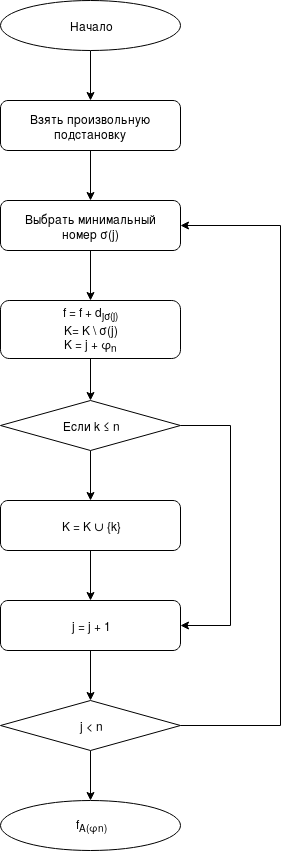
\includegraphics[width=\linewidth, height=\textheight,keepaspectratio]{Chapters/image/flowchart.png}
  \caption{A boat.}
  \label{fig:flowchart}
\end{figure}

\section{Комментарии к алгоритму}
Асимптотическое поведение трехиндексной аксиальной задачи о назначениях значительно отличается от поведения 
классической задачи о назначениях. В ряде статей Grundel Krohmal Oleveira было изучено поведение ожидаемого значения  оптимальной функции. Ими было доказано, что оно стремится к левой границе распределения весовых коэфициентов.

Теорема
При $b_n / a_n = o(n/ \mathrm{ln} n)$ алгоритм является ассимптотически оптимальным для 3-АЗН на классе матриц $М_n$
и его временная сложность  $O(n^2)$.

При $b_n / a_n = o(\mathrm{ln} n)$ алгоритм является ассимптотически оптимальным для 3-АЗН на классе матриц $М_n$
и его временная сложность  $O(n \mathrm{ln} n)$. 

Несмотря на то, что алгоритм показывает полиномиальное время выполения, возможен ряд улучшений
Например, заметно что алгоритм неустойчив относительно выбора начальной перестановки.
Также, 
\section{Вводимые модификации}
\subsection{Генерация нескольких начальных перестановок}
Изменим алгортим следующим образом

Пусть на начальном этапе дается не одна случайная перестановка, 
а $m$. Тогда на выходе можем выбрать лучшую ... Бред
\subsection{Выбор лучшей перестановки}
Введем функционал вида 

При известном точном решении будем говорить, что одна перестановка лучше другой
если она за тоже число шагов будет ближе сходится к точному решению 


\section{Итеративный алгоритм}
Добавим следующие шаги
После последнего шага сохраним результат, пойдем в начало и запустим алгоритм еще раз
Повторим M раз
Получим М выводов, в качестве ответа выберем устредненное значение.  % Algorithm
\chapter{Программная реализация и вычислительный эксперемент}
\section{Описание}
здесь будет алгоритм, вводные данные
\section{Эксперимент}
здесь будут таблицы
 % Algorithm

\addtocontents{toc}{\vspace{2em}}  % Add a gap in the Contents, for aesthetics
\backmatter

%% ----------------------------------------------------------------
\label{Bibliography}
\lhead{\emph{Bibliography}}  % Change the left side page header to "Bibliography"
\bibliographystyle{unsrtnat}  % Use the "unsrtnat" BibTeX style for formatting the Bibliography
\bibliography{Bibliography}  % The references (bibliography) information are stored in the file named "Bibliography.bib"


\end{document}  % The End
%% ----------------------------------------------------------------